\documentclass[11pt]{article}
\usepackage{graphicx}
\usepackage[margin=2.5cm]{geometry}
\usepackage{array}
\usepackage{tabu} 

\title{Project Proposal: Enhancing Social HRI using Affective Communication}
\author{Katie Winkle}

\begin{document}

\maketitle

\section{Aims and Objectives}
\subsection{Aims}
The overall aim of this project is to investigate emotional expression in robot to human communication. Specifically of interest is the potential for robot to human emotion transfer and the potential benefits this might have. This can be expressed as two key project aims:

\begin{enumerate}
\item Investigate robot to human emotion transfer
\item Investigate the impact of affective robot communication
\end{enumerate}

The first aim deals specifically with exploring emotion transfer, i.e. whether a human's emotional state can be changed through interaction with an emotionally expressive robot. The second aim is to demonstrate, regardless of whether emotion transfer occurs, how such emotional expression might impact on human-robot interaction (HRI). Some aspects for consideration are listed under Objective 3 however defining specific evaluation measures is non-trivial and makes up part of the required investigation. Generally it is the impact on the robot's effectiveness that should be considered; however the definition of effectiveness depends on the purpose of the robot. 

\subsection{Objectives}
In order to achieve the project aims, a list of specific objectives has been derived as follows: 
\begin{enumerate}
\item Study affective communication and emotion contagion
\item Create a parameterised model for generating emotional robot expression
\begin{itemize}
\item Conduct a model evaluation experiment for refinement
\end{itemize}
\item Conduct HRI experiment(s) to test the effects of affective robot communication
\begin{itemize}
\item Consider human/robot task performance and human emotional state
\end{itemize}
\end{enumerate}

\section{Motivation}
The psychological phenomenon of interpersonal emotion transfer (IET) between humans is still not fully understood; however it is believed to include social appraisal and emotion contagion effects \cite{parkinson2011interpersonal}. In this context social appraisal describes a person's judgement of something being affected by the emotional response of another (i.e. affecting what they think), whereas emotion contagion describes a change in their emotional state (i.e. affecting how they feel). For example, it has been demonstrated that listening to a neutral text spoken happily or sadly can induce similar feelings in the listener \cite{neumann2000mood} and that the same household object will be rated differently if it is presented alongside a picture of a smiling or disgusted face \cite{bayliss2007affective}. In addition, there is growing evidence that nonverbal emotional expression is an important and subconscious part of human communication which has evolved as a mechanism for quickly communicating a range of information such as social status and level of threat (see \cite{tracy2015nonverbal} for a review). 

Based on this there are at least two major reasons for wanting to design a robot with IET capabilities. Firstly, if emotional expression is an important part of human communication, then a robot with such capabilities might be more lifelike, more likeable and more natural to interact with. Secondly, the effects of IET described above, e.g shaping people's judgement or decision making and impacting on how they feel might be beneficial in a range of HRI applications just as it is in human-human interaction (HHI). In fact, example HRI scenarios where emotional expression might be useful might follow directly from those we can imagine in HHI, e.g. in encouraging children or care of the unwell; applications for which social robots have already been demonstrated (e.g. \cite{shiomi2015can}, \cite{gockley2006encouraging}). As one speculative example, endowing an social assisted living robot with IET  capabilities might offer the following functionality benefits: 
\begin{itemize}
\item the robot could provide more realistic and enjoyable social companionship
\item the robot could `cheer up' the user by being cheerful itself
\item the robot could give the user a positive impression of potentially undesirable tasks, e.g. taking medication or doing exercise
\item the robot could provide more effective encouragement during activities like those above
\item the robot could appear empathetic and caring, leading to a better human-robot relationship
\end{itemize}

However, this reasoning assumes that IET occurs equally well in HRI as HHI and that the effects on the human partner would be the same as if it was a human rather than a robot they were interacting with. Arguably, given the well known effect of the `uncanny valley' \cite{mori2012uncanny}; this assumption might not be valid and hence warrants further study. Research done so far suggest demonstrates that recognisable emotional expression is certainly possible in a range of robots (e.g. X X X from lit review), however the impact of this on a human's own emotional state and the robot's effectiveness is less well documented. 

In summary, the potential benefits of robot emotional expression and robot to human IET are clear. However, there is still significant uncertainty and a lack of evidence surrounding whether IET from a robot to a human can occur  and, if so, what impact this might have on the robot's effectiveness and/or the human's task performance. Addressing this uncertainty and lack of evidence in order to evaluate the real-world potential of robot-human IET forms the main motivation for undertaking this project. 

\section{Literature Review}
\subsection{IET and Emotional Expression in Humans}
There are different hypotheses concerning the purpose of IET and emotional expression more generally in HHI. A functionalist approach (considering the consequences in order to determine the purpose) suggests that at the dyadic level, emotion expressions help individuals determine other's emotions, beliefs, intentions and orientation towards their relationship (i.e. dominant or submissive); and that evoking emotions in others is associated with behaviours such as avoidance, helping, affiliation and soothing \cite{keltner1999social}. An evolutionary approach (considering development over time and the link to population fitness) suggests that emotional expression evolved from being a physiological response (e.g. scrunching the nose to prevent inhalation of noxious gas) into a form of social communication, which observers evolved an ability to instantly and subconsciously decode in order to obtain information about the expresser and/or their environment \cite{shariff2011emotion}. One consistent theme in the psychology literature however is the importance and subconscious nature of IET resulting from emotional expression in communication, and this is what has the most potential for use in HRI. 

There is evidence to suggest that one form of IET is social appraisal, whereby individual human judgement is influenced the perceived judgement of others \cite{parkinson2011interpersonal}. Specifically it has been demonstrated that judgement of an everyday object is different depending on whether it is presented alongside a smiling or disgusted face \cite{bayliss2007affective} which suggests that emotional expression is a trigger for this form of IET. Another experiment demonstrated that even in a very dangerous situation (a simulated fire) participants surrounded by seemingly calm and unresponsive actors were slower to react than participants that were alone; it has been argued that this could be due to IET effects whereby the participants felt calmer due to the calmness of the actors and also judged the situation to be less dangerous based on their percieved lack of concern (\cite{latane1968group} as discussed in \cite{parkinson2011interpersonal}).

Another evidenced form of IET is emotion contagion, whereby an individual's emotional state changes to based on that of their interaction partner; however this is less well understood and more difficult to experimentally examine than social appraisal effects \cite{parkinson2011interpersonal}. There is a general consensus that most emotion contagion is a form of social mimicry, however it is disputed whether this is based on physical mimicry in which the related emotion is generated from mimicking the physical expression; i.e. the individual smiles in response to a smile and hence feels happier \cite{strack1988inhibiting}, or whether expression is less important and actually an individual must understand and perceive the reason for another's emotional expression in order for emotion contagion to occur \cite{tamietto2009unseen}. In contrast to the idea of simple mimicry however it should also be noted that emotion contagion has been demonstrated to induce contrasting rather than matching emotions, and that this may be linked to social stature \cite{tiedens2003power}.

Demonstrated examples of emotion contagion highlight the impact it can have both at the individual and group level. For example, listening to neutral information spoken in an emotional way can induce similar emotions in the listener \cite{neumann2000mood}, and emotion contagion in a group can improve attitudes and reduce conflicts resulting in improved task performance \cite{barsade2002ripple}. It has even been demonstrated that emotion contagion can occur through social networks with Facebook users producing more positive or negative posts when the amount of negative or positive emotional content in their newsfeed was reduced \cite{kramer2014experimental} respectively. Other interesting results include thirsty individuals pouring more or less from a drink jug if exposed to a smiling or frowning face respectively \cite{winkielman2005unconscious} or acceptance of an offer being higher for smiling and lower for frowning proposers compared to those that wore neutral expressions \cite{mussel2013value}. 

In summary there is clear evidence that, whilst the origins and exact mechanisms of IET are not clear, it has significant impact on HHI and can influence an individual's feelings, judgement and behaviour as well as group collaboration and effectiveness. This surely warrants the study of IET in HRI in order to establish whether the same effects can be observed, and if so whether they can be useful e.g. in improving robot design (trying to say how much people like them?) or in improving task performance. Key research questions are whether robot to human IET can occur and how robot emotional expressions affect humans' judgements and behaviour. Additionally the ability to experiment with individual elements of emotional expression in a controlled way, as possible on a robotic platform, might be useful in demonstrating and contributing to some of the theories on IET in the psychology literature. 

In order to design emotionally expressive robot behaviours it must first be established how emotion is expressed in humans and identify specific behaviours which might be transferable onto a robot. Specifically the robotic platform to be used for this project is Aldebaran Robotics' humanoid robot NAO [REFERENCE OR FOOTNOTE MAYBE?], which means that facial expression cannot be altered and hence lies outside the scope of this project.  As such, the following discussion covers emotional expression through speech and movement only. It is noted however that the literature describes facial expression as an important part of affective communication and so further work in the future would be to extend the investigation proposed here to include that.

The study of emotion recognition in point light displays generated from emotional dance and acting performances has demonstrated that movement alone can express emotion even if the semantic purpose of that movement is unknown (e.g. \cite{dittrich1996perception}, \cite{pollick2001perceiving}, \cite{atkinson2004emotion}). Laban Movement Analysis (LMA), a multidisciplinary tool for movement analysis considering parameters such as weight, space and time, has become a standard method for parameterising movement in order to further study such effects \cite{lab2011}. As such, instructions on how to perform a certain emotion, as might be explained to dancers or actors, typically utilise LMA (e.g. \cite{newlove1993laban}). Similarly it is widely accepted that emotion can be portrayed through neutral speech \cite{neumann2000mood} or across languages \cite{scherer2000cross} and similar to LMA, this can be quantitatively described by variation in parameters such as pitch, speed and quality (e.g. \cite{scherer1986vocal}, \cite{cowie2001emotion}). One important conclusion from these findings is that emotion can theoretically be expressed through any movement or speech, regardless of semantic content. This is particularly relevant for robotiscists because it means that emotional expression can be added to communication or task execution without changing the robot's functional behaviour. In conclusion, the reviewed literature suggests that this project's objective to use a parameterised model for generating emotional expression is appropriate and offers a significant set of specific parameters that should be experimented with.

\subsection{(current/previous?)Emotional Expression and IET in Robots}
Giving robots the capability to display emotional expressions has been a recurrent theme in social robotics since the field's infancy [breazel reference]. Recent demonstrations include robots whose emotional state and hence behaviour is adaptive based on such things at its 'personality', 'loyalty' to the user or whether it is winning or losing at a game [REFERENCES] Whilst adaptive emotional expression is certainly an area of further work for this project, the initial concern is simply the parameterised generation of pre-determined emotions which can be displayed through non-specific functional behaviours. Examples of such a framework have already been demonstrated and are clearly of particular relevance to this project. Three such models, all inspired by the human emotional motion and voice parameterisation discussed in the previous subsection, have been identified for further discussion below.  

Masuda and Koto's system uses the six main parameters of LMA: space, time, weight, inclination, height and area, which are set based on previous analysis of observed movement emotion classification from a pilot experiment \cite{masuda2009emotion}. Implemented on a humanoid robot the resulting motion had an average emotion recognition rate greater than 60\% \cite{masuda2010motion}. Lim et al.'s framework for adding emotion to gesturing uses four parameters: speed, intensity, regularity and extent, which are set based on a mapping from the same features measured in a speech sample. Implemented on a NAO the resulting motion had an emotion recognition rate of above 60\% and, when combined with the original speech sample, lead to improved recognition rates for the emotions of happiness and sadness compared to speech alone \cite{lim2011converting}. Xu et al.'s framework uses a combination of general motion and pose parameters (e.g. speed, decay rate, stroke curves) as well as gesture specific ones (e.g. palm up or down). In addition the head is utilised as an effector which can be set in different poses. Parameter settings were then derived by averaging the results of an experiment in which participants were asked to set them in order to achieve specific emotional expressions on a NAO \cite{xu2013mood}. A later experiment demonstrated that different arousal and valence states can be recognised based on these parameters however no results for specific emotion recognition were described \cite{xu2013bodily}.

Considering these three models, Lim et al.'s is the most simple and yet it achieved very similar recognition rates to Masuda and XXX and the idea of setting parameters based on feature matching to speech samples could result in more natural resulting behaviour. It would need to be investigated how well this feature matching would work on artificially generated speech rather than actor samples, because in that case the effectiveness of the whole system would essentially be linked to how well the generated speech can portray emotion. However, if the parameters could be set in a different way then the concept of having a small number of generic parameters that map directly onto both speech and motion could form the basis of a simple yet powerful framework for easily generating complete and natural emotional expressions. Xu et al.'s method of essentially crowd-sourcing parameter settings for different emotions could be explored as such an alternative option. Additionally, Xu et al.'s use of the head as a independent end effector for emotion generation, whilst quite separate to the key parameterisation concept, may be worth investigating. 

Of these three models only Xu et al. went on to evaluate the impact of their generated emotional expression on HRI \cite{xu2014robot}. There have been other such studies designed to demonstrate the potential impact of emotional expression on HRI however, although they typically provide less detail on the mechanism for behaviour generation. One key objective of this project is to undertake experiment(s) in order to investigate the HRI impact of the proposed parameterisation model, therefore the evaluation criteria for such demonstrations is worthwhile of discussion as presented in the following subsection.

\subsection{Experimentally Evaluating the Impact of Affective Communication}

Previous studies documenting the impact of affective robot communication have typically produced only qualitative data. For example, Tielman et al. demonstrated an adaptive emotion model implemented on a NAO used to play a quiz game with children; by using questionnaires they determined that children found emotional expression to be a positive trait for a robot \cite{tielman2014adaptive}. Similarly a long term study documenting the use of a humanoid game playing robot in an elderly care home found, also by questionnaire, that emotional expression was voted a top ranking positive trait by the users \cite{louie2012playing}. Clearly such qualitative results are important and can offer a valuable insight into HRI, especially surrounding how well 'liked' the robot is which is some measure of the robot's effectiveness itself, however examples from the psychology literature suggest that it should also be possible to produce more quantitative results which demonstrate the measured impact of affective communication, e.g. around the performance of a task \cite{barsade2002ripple} or reaction to an event \cite{latane1968group}.

In a rare example of quantitative study considering robot to human IET, Xu et al. demonstrated that participants performed better in a hard task when working with a robot displaying a negative rather than positive 'mood'; they then used this result to argue that emotion  contagion had occurred because of a known psychological phenomenon that humans undertake certain types of task better when in a negative mood \cite{xu2014robot}. Finding further inspiration for evaluation methods and experiment design requires the consideration of HRI studies that do not specifcally consider affective communication but do measure the impact of different robot behaviours. Two such studies are outlined below.

Chidambaram et al. used a desert survival HRI task to demonstrate how both vocal and nonverbal robot cues affected its persuasiveness \cite{chidambaram2012designing}. They used a range of conditions considering variation or lack thereof in body movement (proximity, gaze and gesturing) and voice (monotone or varied pitch). Their evaluation measures combined subject surveys of perceived persuasiveness and objective measures of compliance with the robots suggestions to measure actual persuasiveness. This had the advantage of allowing a valuable comparison between actual and perceived persuasion results to be made in the discussion. Nakagawa et al. used a monotonous task with a robot companion to determine the effect of robot touch on motivation \cite{nakagawa2011effect}. Participants were asked to undertake a monotonous task for as long as they liked, the base condition had the robot simply talking as a companion, the two other condition involved the robot being passively touched by and actively touching the participant while they worked. The time spent undertaking the task was measured for each condition to give a quantitative measure of the impact of robot touch on motivation. Similar to the work of Chidambaram et al., subjective feedback measures were also used to collect information on the participants perception but in this case of the robot generally rather than specifically its use in motivation. 

In summary there are very few previous HRI studies that deal specifically with the impact of affective communication, however inspiration can be drawn from other HRI and HHI/psychology studies. In fact, how best to demonstrate the impact of affective communication is one of the key research questions posed in this project; the aim is to generate insightful data that offers some quantitative measure of impact but also captures more qualitative information to allow for interesting discussion. As listed under Objective 3, key aspects for consideration are human/robot task performance and human emotional state, however further investigation is required alongside experiment design in order to create effective evaluation measures for capturing any impact in these areas.

\section{Risk Register}
%\begin{tabu} to \textwidth { | X[l] | X[l] | X[c] | X[c] | X[c] | }
%\begin{tabular}{|c|c|c|c|c|}
\begin{center}
	\begin{tabular}{|m{6cm}|m{5cm}|m{1.8cm}|m{1cm}|m{1cm}|}
		\hline
		Risk & Mitigation & Likelihood & Impact & \textbf{Score} \\
		\hline
		Emotion generation model not ready in time for final experiment & Hand script behaviours to allow experiment to go ahead & 2 & 3 & \textbf{6} \\ 
		\hline 
		Issue with hardware of robot platform preventing experiment being undertaken & Some time in plan for rescheduling, or could implement reduced experiment using virtual agent & 2 & 3 & \textbf{6} \\
		\hline
		Identified emotional behaviours from literature do not transfer onto robot platform & Identify many alternative behaviours and form a prioritised list to work through and test, consider the most 'simple' emotions first & 2 & 4 & \textbf{8} \\ 
		\hline 
		Cannot recruit enough participants for statistical significance in experiment(s) & Start recruiting in sensible advance of experiment, use within rather than between subject experiment design, consider virtual alternatives such as video surveys & 3 & 3 & \textbf{9} \\
		\hline
	\end{tabular} 
\end{center}
%\end{tabu}

\section{Timeline}
A Gantt Chart showing key project activities and their suggested time allocations is given in Figure \ref{fig:ProjectTimeline}. 

\begin{figure}
\centering
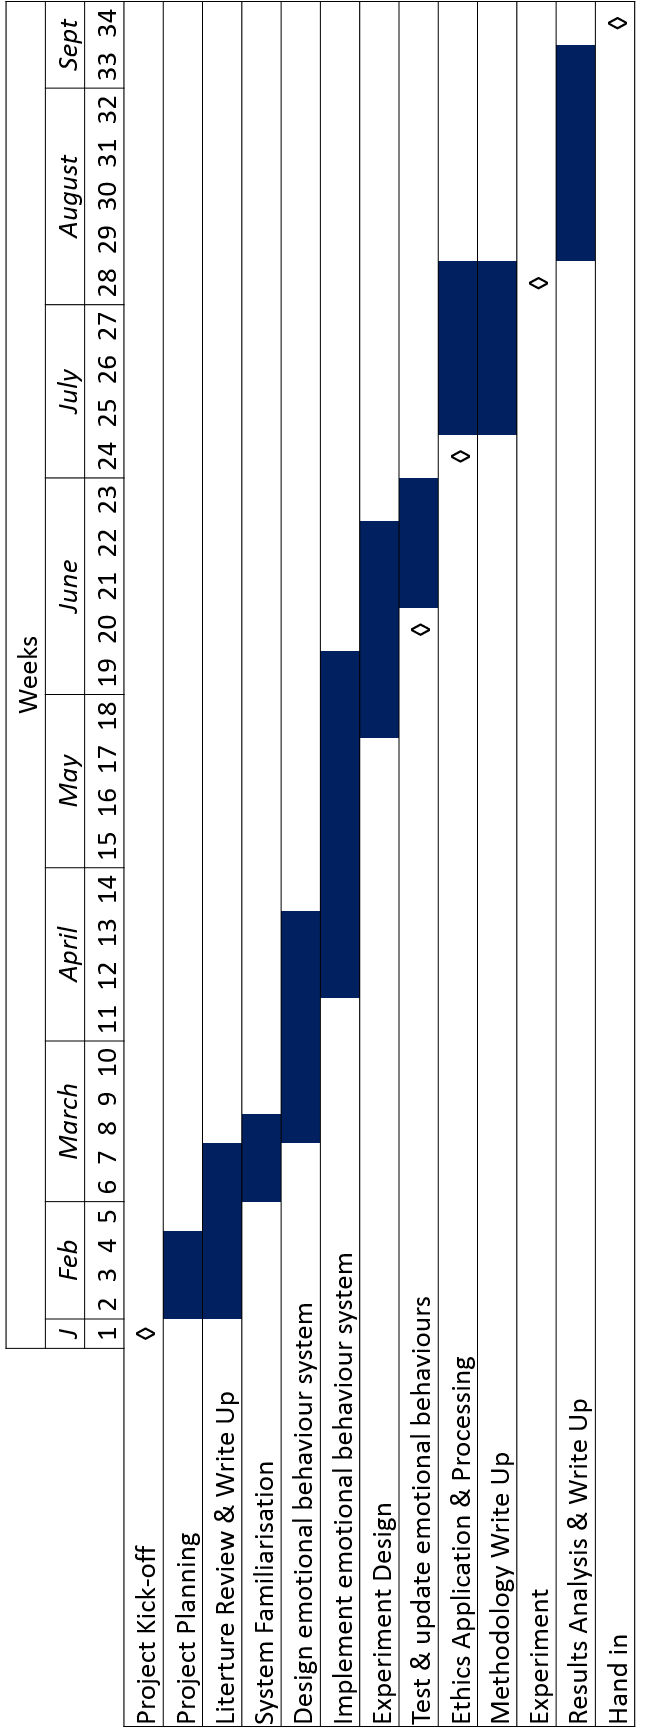
\includegraphics[height=0.9\textheight,]{ProjectTimeline2.png}
\caption{Project timeline - diamonds indicate discrete timing point events.}
\label{fig:ProjectTimeline}
\end{figure}

\bibliographystyle{unsrt}
\bibliography{ProjectReferences}
\end{document}
